\apendice{Documentación de usuario}

\section{Requisitos software y hardware para ejecutar el proyecto.}

\subsection{Requisitos software}

Las librerías necesarias para este proyecto se encuentran al principio del proyecto para su instalación en servicios en linea con aceleración de GPU pero en el caso de su instalación en local se encontrarán en el archivo requirements.txt, también para ejecutarlo en local se deberá tener Python y pip instalado %TODO Crear el archivo requirements.

\subsection{Requisitos hardware}

No se recomienda la ejecución en local del programa, sin embargo se ha realizado una medición de la gpu necesaria para ejecutar el proyecto ya que es el aspecto más exigente, se puede ver en la figura \ref{fig:hardware}.


\begin{figure}[h!]
    \centering
    \includegraphics[width=1\textwidth]{img/reqhard.png}
    \caption{Requisitos de GPU}
    \label{fig:hardware}
\end{figure}

\section{Instalación / Puesta en marcha}

Debido a que no se creó un espacio en Hugging Face que pueda soportar de forma permanente los grandes requisitos de GPU del proyecto se recurre a demos temporales.

Para visualizar la prueba de concepto simplemente hay que ejecutar el código presente en el repositorio en un entorno con suficiente GPU, por ejemplo, Kaggle o Google colab y acceder al link que se creará al final de la ejecución.

Para su puesta en marcha en local se deberá clonar el repositorio en github e instalar en el entorno deseado el archivo requirements.txt con el siguiente comando pip install -r requirements.txt siempre y cuando se tenga instalado tanto Python como pip en el sistema.


\section{Manuales y/o Demostraciones prácticas}

En este ejemplo se ejecutará el proyecto desde google colab empleando la aceleración por hardware T4 la cual será suficiente para la ejecución del proyecto, esto se podrá seleccionar desde la opción en el panel superior Entorno de ejecución -> Cambiar tipo de entorno de ejecución  y seleccionar un acelerador por hardware suficiente para ejecutar el proyecto, T4 es suficiente como se ve en la figura \ref{fig:aceleracion}.


\begin{figure}[h!]
    \centering
    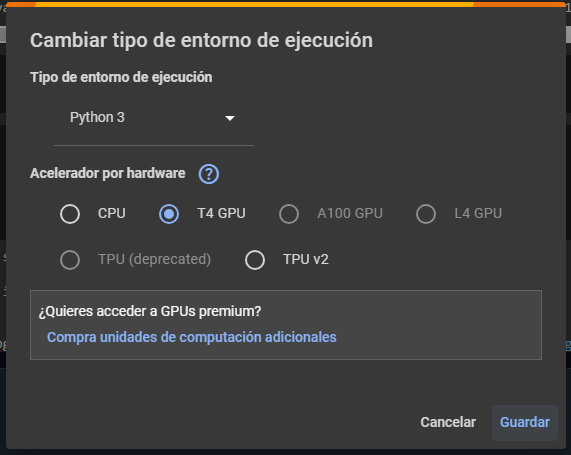
\includegraphics[width=1\textwidth]{img/aceleracion.png}
    \caption{Demostración de aceleración por hardware}
    \label{fig:aceleracion}
\end{figure}


Una vez ejecutado el proyecto se abrirá al final una ventana con la que se podrá interactuar con el modelo y un link con el que se podrá interactuar con el en línea y compartirlo para que se pueda acceder a él desde distintos dispositivos, el ejemplo de la interfaz vacía se puede ver en la figura \ref{fig:guivacia}.

\begin{figure}[h!]
    \centering
    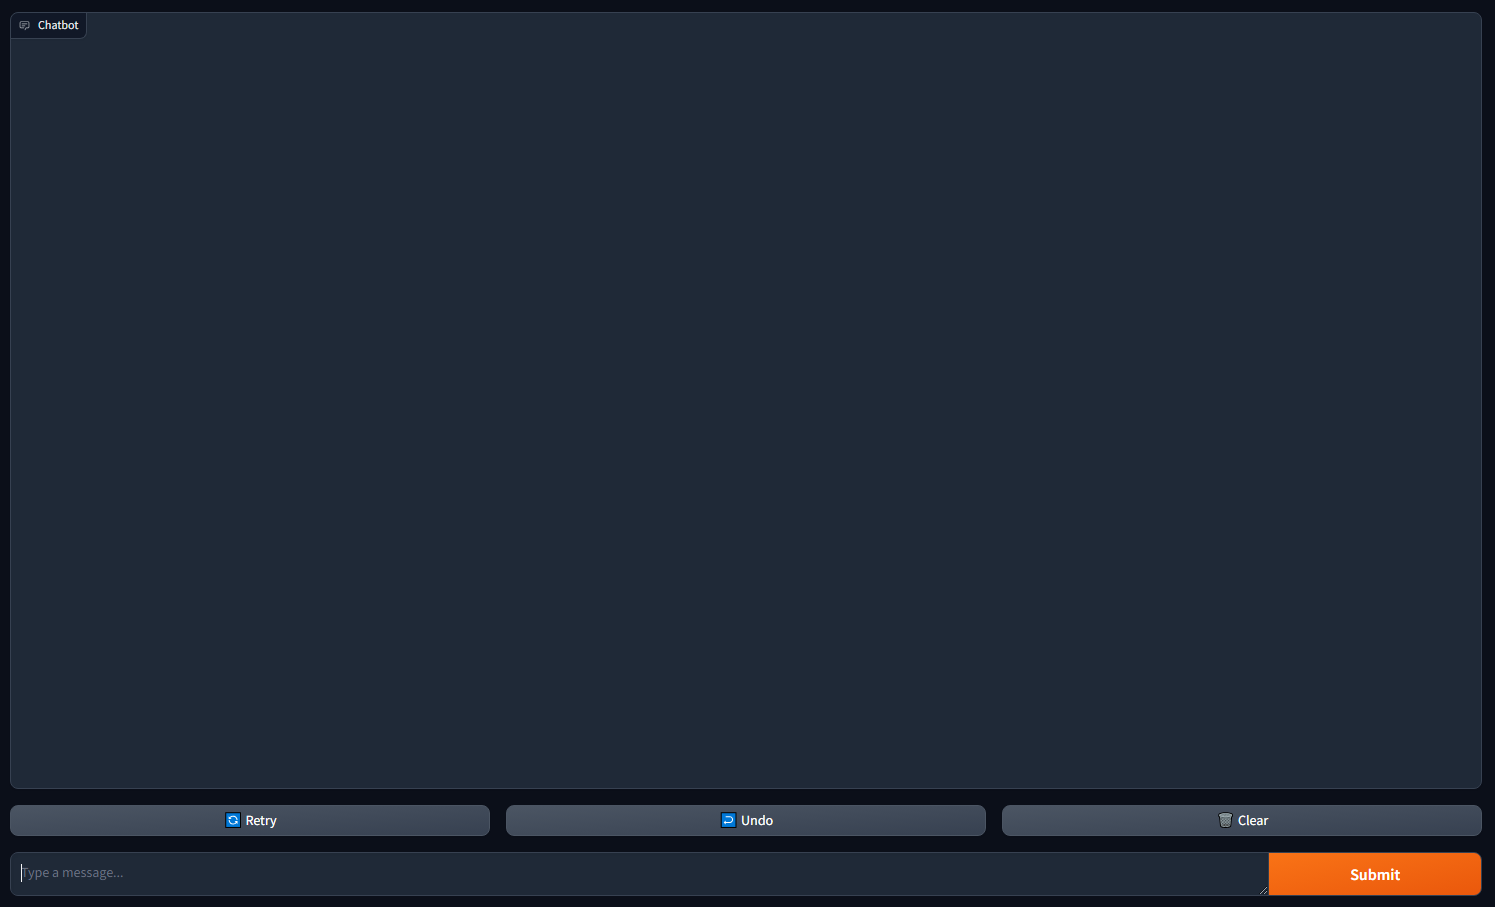
\includegraphics[width=1\textwidth]{img/guivacia.png}
    \caption{Interfaz gráfica de usuario}
    \label{fig:guivacia}
\end{figure}

Una vez ejecutada simplemente falta insertar el prompt deseado y seleccionar submit, luego, el modelo arrojará una respuesta con los abstracts que haya interpretado como los más relevantes según el prompt del usuario y la respuesta del prompt enriquecido con dichos abstracts obteniendo así la salida esperada de la respuesta al prompt inicial y bibliografía que la apoye, se puede ver en la figura \ref{fig:guirellena}

\begin{figure}[h!]
    \centering
    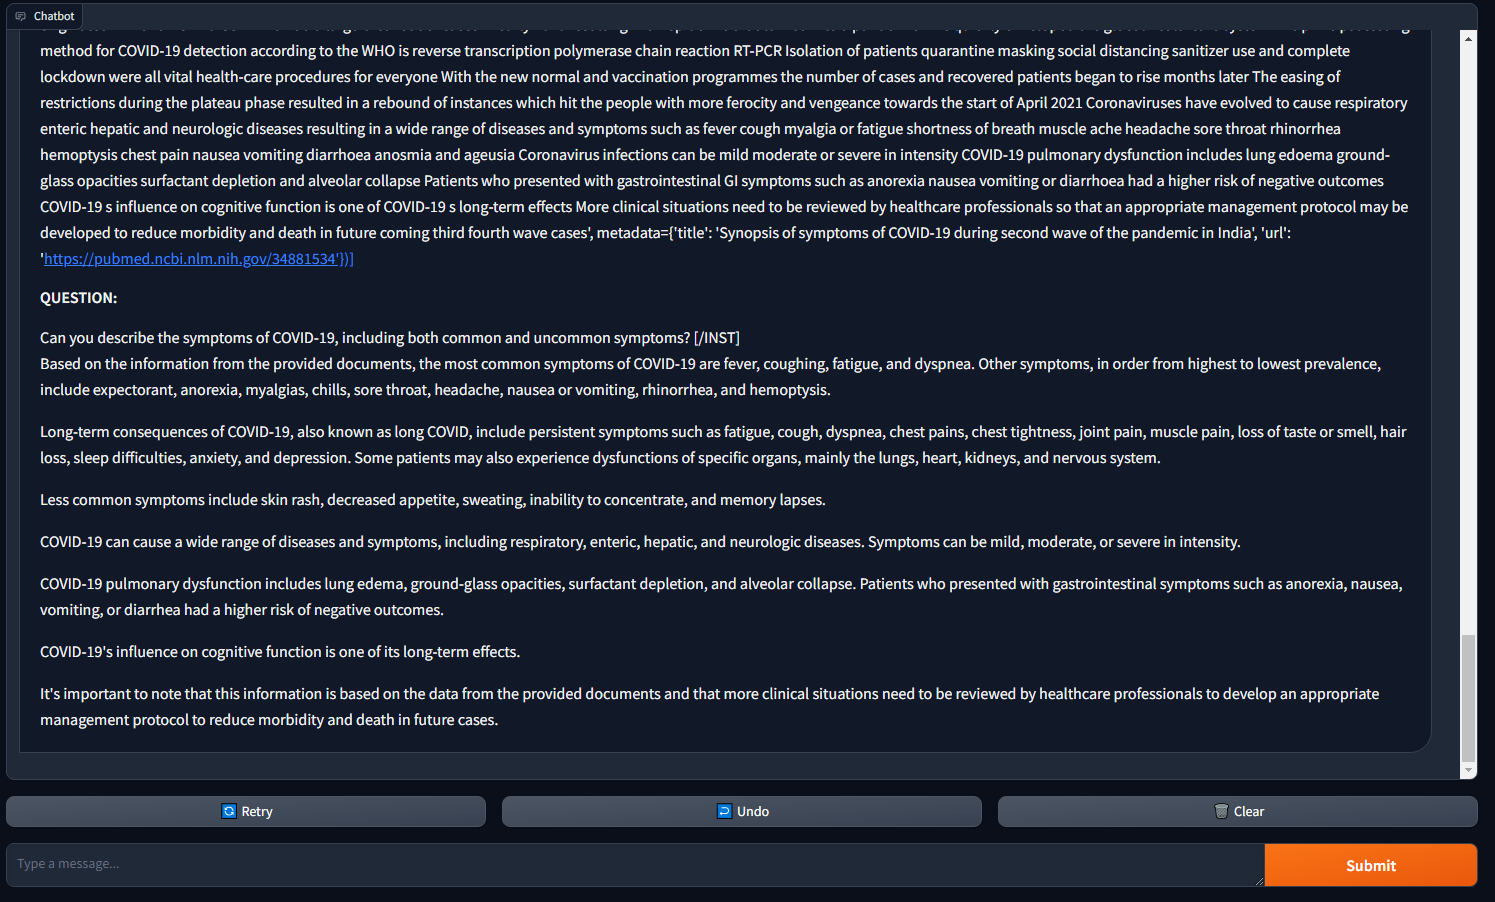
\includegraphics[width=1\textwidth]{img/guirellena.png}
    \caption{Interfaz gráfica de usuario tras una ejecución}
    \label{fig:guirellena}
\end{figure}